
In the continuity of \citet{fintzi2024buoyancy} we study the microstructure of emulsion using the \textit{Nearest-Particle Statistics} (NPS) framework. 
Particularly, we will be interested in the age-included nearest-pair probability density function \citep{zhang2021ensemble}. 
In addition to give details about relative positions this probability density provides information regarding the time of interaction between the nearest particle pairs. 

\subsection{The age-included nearest-pair probability density function}
Let $P(\FF)$ be the probability density function that describes the probability of finding the flow in the configuration $\FF$.
Then, we define $d\mathscr{P} = P(\FF)d\FF$ as the probable number of realizations in the incremental region of the flow' phase space, $d\FF$ around $\FF$.
The vectors  $\textbf{x}_i(t,\FF)$ and $\textbf{x}_j(\FF,t)$ refer to the position of the particles $i$ and $j$ at time $t$ for a configuration $\FF$, respectively. 
Additionally, the time $t_{ij}(\FF)$, is the time at which the particles $i$ and $j$ became nearest neighbor.
This Lagrangian quantity is a constant scalar fixed in time and may change according to the flow configuration $\FF$.
Based on these Lagrangian quantities we can define The age-included nearest pair distribution function as \citep{zhang2023evolution},
\begin{equation}
    P_{nst}(\textbf{x},\textbf{r},a,t) =
    \int \sum_{i}^{N_b}\delta[\textbf{x}-\textbf{x}_i(t,\FF)]
    \sum_{j\neq i}^{N_b}\delta[\textbf{x}+\textbf{r}-\textbf{x}_j(t,\FF)]
    \delta[t+a-t_c^{ij}(\FF)] 
    h_{ij} (t,\FF)
    d\mathscr{P},
    \label{eq:P_nstij}
\end{equation}
where
\begin{equation*}
    h_{ij}(\FF,t)
    = \left\{
        \begin{tabular}{cc}
            $1/N_i(\FF,t)$ & if $j$ is one of the $N^{th}$ nearest neighbors of $i$ \\
            0& otherwise
        \end{tabular}
        \right.,
\end{equation*}
Here $\textbf{x}$ and $\textbf{r}$ are coordinate vectors in $\mathbb{R}^3$ and $a \geq 0 $ is the \textit{age} of interaction, i.e. the current time minus the time at which both particle became nearest neighbors.   
With this definition $P_{nst}(\textbf{x},\textbf{r},t,a)$ is the probability of finding a particle at \textbf{x} and time $t$, with a nearest neighbor at the position $\textbf{x}+\textbf{r}$ with age $a$.
We also introduce the \textit{reduced} nearest neighbor distributions, they read as
\begin{align}
    P_\text{r}(\textbf{r}|\textbf{x},t)
    =\frac{1}{n_p(\textbf{x},t)}\int_0^\infty P_\text{nst}(\textbf{x},\textbf{r},t,a) da,\\
    P_a(a|\textbf{x},t)
    = \frac{1}{n_p(\textbf{x},t)}\int_{\mathbb{R}^3} P_\text{nst}(\textbf{x},\textbf{r},t,a) d\textbf{r},
\end{align}
where $P_r(\textbf{r}|\textbf{x},t)$ represents the probability of finding a nearest neighbor at $\textbf{x}+\textbf{r}$ knowing that a particle is already present at \textbf{x} and time $t$, regardless of the age of interaction. 
And $P_a(a|\textbf{x},t)$ is the probability of finding  a nearest-neighboring particles having age $a$, regardless of the relative position, knowing a particle is present at \textbf{x} and time $t$. 
Note that these distribution functions are all normalized such that 
\begin{equation}
    \frac{1}{n_p(\textbf{x},t)}\int_0^\infty \int_{\mathbb{R}^3} P_\text{nst}(\textbf{x},\textbf{r},t,a) d\textbf{r} da 
    = 
    \int_{\mathbb{R}^3} P_\text{r}(\textbf{x},\textbf{r},t) d\textbf{r} 
    = \int_0^\infty P_\text{a}(\textbf{x},\textbf{r},t) da 
    = 1,
    \label{eq:norm}
\end{equation}
with $n_p(\textbf{x},t)$ the number density function, defined as
\begin{equation}
    n_p(\textbf{x},t)= 
    \int \sum_{i}^{N_b}\delta[\textbf{x}-\textbf{x}_i(t,\FF)] d\mathscr{P}.
    \label{eq:n_p}
\end{equation}


In addition to these distribution functions we also wish to analyze the relative kinematic between nearest neighbors. 
To that end we introduce the Lagrangian relative velocity $\textbf{w}_{ij}(t,\FF) = \textbf{u}_j(t,\FF) - \textbf{u}_i(t,\FF)$, with $\textbf{u}_i(t,\FF)$ and $\textbf{u}_j(t,\FF)$, the center of mass velocity of the particle $i$ and $j$, respectively.
The conditional average of the Lagrangian relative velocity can be written
\begin{equation*}
    \textbf{w}^\text{nst}_p (\textbf{x},\textbf{r},t,a)
    = 
    \frac{1}{P_{nst}(\textbf{x},\textbf{r},t,a)}
    \int \sum_{i}^{N_b}\delta(\textbf{x}-\textbf{x}_i)
    \sum_{j\neq i}^{N_b}\delta(\textbf{x}+\textbf{r}-\textbf{x}_j) 
    \delta(t+a-t_c^{ij}) 
    \textbf{w}_{ij}
    h_{ij} 
    d\mathscr{P}.
    \label{eq:q_nstij}
\end{equation*}
Following this definition, $\textbf{w}^\text{nst}_p(\textbf{x},\textbf{r},t,a)$ is the averaged relative velocity between two nearest neighboring particles, one of which is situated at $\textbf{x}$ and time $t$, with its nearest neighbor at $\textbf{x}+\textbf{r}$ with age $a$. 
The physical meaning of such a field will be further investigated in \ref{sec:velocity}. 
For instance, note that the subscript $_p$ indicates that $\textbf{w}^\text{nst}_p$ is at the origin a Lagrangian property, it is therefore averaged conditionally on the presence of a particle at $\textbf{x}$ and time $t$. 
Whereas superscript $^\text{nst}$ indicates that $\textbf{w}_{ij}(\FF,t)$ is conditionally averaged on the presence of a nearest neighbor at $\textbf{x}+\textbf{r}$ with age $a$. 

In general, $\textbf{w}_{ij}(t,\FF)$ can be replaced by any particle's properties. 
An example particularly interesting in this work is the particle absolute velocity $\textbf{u}_i(\FF,t)$.
In this case, $\textbf{u}^\text{nst}_p(\textbf{x},\textbf{r},t,a)$ represents the averaged velocity of the particles, given that a particle is present at \textbf{x} and time $t$, with its nearest neighbor located at $\textbf{x}+\textbf{r}$ with age $a$. 
Using the property of the nearest neighbor distribution functions we deduce that  $\textbf{u}^\text{nst}_p$ is related to the ensemble averaged particle phase velocity, defined as 
\begin{equation*}
    \textbf{u}_p(\textbf{x},t)=\frac{1}{n_p(\textbf{x},t)} 
    \int \sum_{i}^{N_b}\delta[\textbf{x}-\textbf{x}_i(t,\FF)]  \textbf{u}_i(t,\FF)d\mathscr{P},
\end{equation*}
through the relation
\begin{equation}
    \textbf{u}_p = \frac{1}{n_p(\textbf{x},t)} \int_0^\infty \int_{\mathbb{R}^3} \textbf{w}_p^\text{nst} P_\text{nst}(\textbf{x},\textbf{r},t,a) d\textbf{r} da. 
    \label{eq:u_p}
\end{equation}



\subsection{A transport equation to describe the evolution of the microstructure}

In our previous work \citep{fintzi2024buoyancy} we have seen that the tensor,
\begin{equation}
    \textbf{R}(\textbf{x},t)
    = \frac{1}{n_p(\textbf{x},t)}
    \int_0^\infty 
    \int_{\mathbb{R}^3}
    \textbf{rr}
    P_\text{nst}(\textbf{x},\textbf{r},a,t)
    d\textbf{r}
    da
    \label{eq:R}
\end{equation}
is able to describe the particles arrangements, or microstructure.
Specifically, it was shown that $\textbf{R}(\textbf{x},t)$ measures features such as layers or clusters of particles. 
The scalar $R = \bm\delta:\textbf{R}(\textbf{x},t)$ with $\bm\delta$ the unit tensor, represents the averaged mean square distance to the nearest neighbors.
And the deviatoric part of this tensor, namely $\textbf{A} = \textbf{R}-\frac{1}{3}R\bm\delta$, measures the anisotropy of the microstructure. 
\ref{fig:scheme_clusters} provides a concise explanation of the implications of the values of $\textbf{A}$ and $R$ on the microstructure.  
And \ref{fig:A} provides phase diagram of the value of $\textbf{A}$ and $R$ obtained in our previous study. 
\begin{figure}[h!]
    \hfill
\begin{tikzpicture}
    \draw[<->] (-1.5,1)node[right]{$y$}--++(0,-1)--++(1,0)node[right]{$x$};
    % \draw[->] (-1,2.5)--++(0,-2)node[midway, left]{$\textbf{g}$};
    \foreach \i in {1,...,5} {
    \pgfmathsetmacro{\x}{rnd}
    \pgfmathsetmacro{\y}{rnd}
    \draw[fill=gray!50] ($(\x,\y)$) circle (0.1);
    }
    \foreach \i in {1,...,5} {
    \pgfmathsetmacro{\x}{rnd}
    \pgfmathsetmacro{\y}{rnd}
    \draw[fill=gray!50] ($(\x+1,\y)$) circle (0.1);
    }
    \foreach \i in {1,...,5} {
    \pgfmathsetmacro{\x}{rnd}
    \pgfmathsetmacro{\y}{rnd}
    \draw[fill=gray!50] ($(\x+2,\y)$) circle (0.1);
    }
    \foreach \i in {1,...,5} {
        \pgfmathsetmacro{\x}{rnd}
        \pgfmathsetmacro{\y}{rnd}
        \draw[fill=gray!50] ($(\x+1,\y+1)$) circle (0.1);
    }
    \foreach \i in {1,...,5} {
    \pgfmathsetmacro{\x}{rnd}
    \pgfmathsetmacro{\y}{rnd}
    \draw[fill=gray!50] ($(\x+2,\y+1)$) circle (0.1);
    }
    \foreach \i in {1,...,5} {
    \pgfmathsetmacro{\x}{rnd}
    \pgfmathsetmacro{\y}{rnd}
    \draw[fill=gray!50] ($(\x,\y+1)$) circle (0.1);
    }
    \foreach \i in {1,...,5} {
        \pgfmathsetmacro{\x}{rnd}
        \pgfmathsetmacro{\y}{rnd}
        \draw[fill=gray!50] ($(\x+1,\y+2)$) circle (0.1);
    }
    \foreach \i in {1,...,5} {
    \pgfmathsetmacro{\x}{rnd}
    \pgfmathsetmacro{\y}{rnd}
    \draw[fill=gray!50] ($(\x+2,\y+2)$) circle (0.1);
    }
    \foreach \i in {1,...,5} {
    \pgfmathsetmacro{\x}{rnd}
    \pgfmathsetmacro{\y}{rnd}
    \draw[fill=gray!50] ($(\x,\y+2)$) circle (0.1);
    }
    \draw (1.5,3.4)node[below]{\textit{Case 1}};
    \draw (1.5,0)node[below]{$\textbf{A}\approx \bm 0$ \& $R\approx r_m^2$};
\end{tikzpicture}
\hfill
\begin{tikzpicture}
    \foreach \i in {1,...,5} {
    \pgfmathsetmacro{\x}{rnd*0.4}
    \pgfmathsetmacro{\y}{rnd*0.4}
    \draw[fill=gray!50] ($(\x,\y)$) circle (0.1);
    }
    \foreach \i in {1,...,5} {
    \pgfmathsetmacro{\x}{rnd*0.3}
    \pgfmathsetmacro{\y}{rnd*0.3}
    \draw[fill=gray!50] ($(\x+1,\y)$) circle (0.1);
    }
    \foreach \i in {1,...,5} {
    \pgfmathsetmacro{\x}{rnd*0.3}
    \pgfmathsetmacro{\y}{rnd*0.3}
    \draw[fill=gray!50] ($(\x+2,\y)$) circle (0.1);
    }
    \foreach \i in {1,...,5} {
        \pgfmathsetmacro{\x}{rnd*0.5}
        \pgfmathsetmacro{\y}{rnd*0.5}
        \draw[fill=gray!50] ($(\x+0.5,\y+1)$) circle (0.1);
    }
    \foreach \i in {1,...,5} {
        \pgfmathsetmacro{\x}{rnd*0.4}
        \pgfmathsetmacro{\y}{rnd*0.4}
        \draw[fill=gray!50] ($(\x+2.5,\y+1)$) circle (0.1);
    }
    \foreach \i in {1,...,5} {
        \pgfmathsetmacro{\x}{rnd*0.4}
        \pgfmathsetmacro{\y}{rnd*0.4}
        \draw[fill=gray!50] ($(\x+1.5,\y+1)$) circle (0.1);
        }
    \foreach \i in {1,...,5} {
        \pgfmathsetmacro{\x}{rnd*0.5}
        \pgfmathsetmacro{\y}{rnd*0.5}
        \draw[fill=gray!50] ($(\x,\y+2)$) circle (0.1);
    }
    \foreach \i in {1,...,5} {
        \pgfmathsetmacro{\x}{rnd*0.4}
        \pgfmathsetmacro{\y}{rnd*0.4}
        \draw[fill=gray!50] ($(\x+2,\y+2)$) circle (0.1);
    }
    \foreach \i in {1,...,5} {
        \pgfmathsetmacro{\x}{rnd*0.4}
        \pgfmathsetmacro{\y}{rnd*0.4}
        \draw[fill=gray!50] ($(\x+1,\y+2)$) circle (0.1);
        }
    \draw (1.5,3.4)node[below]{\textit{Case 2}};
    \draw (1.5,0)node[below]{$\textbf{A}\approx \bm 0$ \& $R < r_m^2$};
\end{tikzpicture}
\hfill
\begin{tikzpicture}
    \foreach \i in {1,...,5} {
    \pgfmathsetmacro{\x}{rnd*1.5}
    \pgfmathsetmacro{\y}{rnd*0.2}
    \draw[fill=gray!50] ($(\x,\y)$) circle (0.1);
    }
    \foreach \i in {1,...,5} {
    \pgfmathsetmacro{\x}{rnd*1.5}
    \pgfmathsetmacro{\y}{rnd*0.3}
    \draw[fill=gray!50] ($(\x+1,\y)$) circle (0.1);
    }
    \foreach \i in {1,...,5} {
    \pgfmathsetmacro{\x}{rnd*1.5}
    \pgfmathsetmacro{\y}{rnd*0.3}
    \draw[fill=gray!50] ($(\x+2,\y)$) circle (0.1);
    }
    \foreach \i in {1,...,5} {
        \pgfmathsetmacro{\x}{rnd*1.5}
        \pgfmathsetmacro{\y}{rnd*0.2}
        \draw[fill=gray!50] ($(\x+1+0.5,\y+1)$) circle (0.1);
    }
    \foreach \i in {1,...,5} {
    \pgfmathsetmacro{\x}{rnd*1.5}
    \pgfmathsetmacro{\y}{rnd*0.2}
    \draw[fill=gray!50] ($(\x+2+0.5,\y+1)$) circle (0.1);
    }
    \foreach \i in {1,...,5} {
    \pgfmathsetmacro{\x}{rnd*1.5}
    \pgfmathsetmacro{\y}{rnd*0.1}
    \draw[fill=gray!50] ($(\x+0.5,\y+1)$) circle (0.1);
    }
    \foreach \i in {1,...,5} {
        \pgfmathsetmacro{\x}{rnd*1.5}
        \pgfmathsetmacro{\y}{rnd*0.2}
        \draw[fill=gray!50] ($(\x+1,\y+2)$) circle (0.1);
    }
    \foreach \i in {1,...,5} {
    \pgfmathsetmacro{\x}{rnd*1.5}
    \pgfmathsetmacro{\y}{rnd*0.2}
    \draw[fill=gray!50] ($(\x+2,\y+2)$) circle (0.1);
    }
    \foreach \i in {1,...,5} {
    \pgfmathsetmacro{\x}{rnd*1.5}
    \pgfmathsetmacro{\y}{rnd*0.1}
    \draw[fill=gray!50] ($(\x,\y+2)$) circle (0.1);
    }
    \draw (1.5,3.4)node[below right]{\textit{Case 3}};
    \draw (1.5,0)node[below]{$A_{xx} > 0$ \& $R< r_m^2$};
\end{tikzpicture}
\hfill
\caption{Sketch of three typical particles arrangements observed in buoyant emulsions.
The gray disks represent droplets or particles in a three-dimensional space. 
$r_m^2$ is the mean square distance to a nearest neighbor in a random suspension of hard sphere \citep{zhang2023evolution,fintzi2024buoyancy}.  
(\textit{Case 1: ``homogeneous''}) Homogeneous arrangement of droplets, referred as homogeneous microstructure or just ``homogeneous''.
(\textit{Case 2: ``clusters''}) Isotropic non-homogeneous microstructure where we  observe the presence of ``clusters'', meaning that the particles are close to each other in average.
The opposite scenario, where particles are on average far from each other, also falls into this category. 
(\textit{Case 3: ``layers''}) The non-isotropic non-homogeneous microstructure where we observe the presence of stratified arrangements.
This type of microstructure is refereed to as layered microstructure or just ``layers''. 
}
\label{fig:scheme_clusters}
\end{figure}
\begin{figure}[h!]
    \centering
    \begin{tikzpicture}[scale=0.8]
        \node (img) at (0,0) {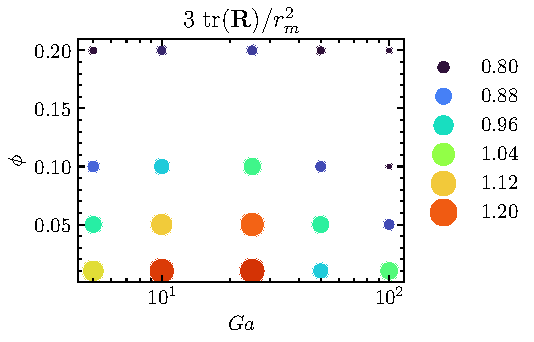
\includegraphics[height=5.5cm]{image/HOMOGENEOUS_NEW/PA/phase_Rtr_l_1.pdf}};
        % \draw[dashed] (10cm,-1.6) ellipse (3 and 2);
        \node (txt) at (-2,1) {Clustering};
        \node (txt) at (-1,-1.6) {Dispersed};
        \draw[dashed] ($(-1,-1.6) + (-10:3 and 2)$(P) arc
        (-10:155:3 and 2);
        \node (img) at (10.5,0) {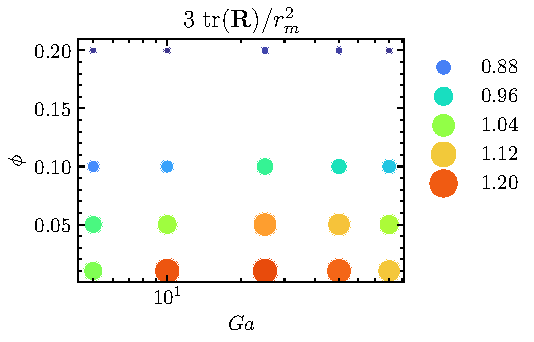
\includegraphics[height=5.5cm]{image/HOMOGENEOUS_NEW/PA/phase_Rtr_l_10.pdf}};
        % \draw[dashed] (10cm,-1.6) ellipse (3 and 2);
        \node (txt) at (8.5,1) {Clustering};
        \node (txt) at (10,-1.6) {Dispersed};
        \draw[dashed] ($(10,-2) + (-10:3 and 2)$(P) arc
        (-10:180:3 and 2);
    \end{tikzpicture}
    \begin{tikzpicture}[scale=0.8]
        \node (img) at (0,0) {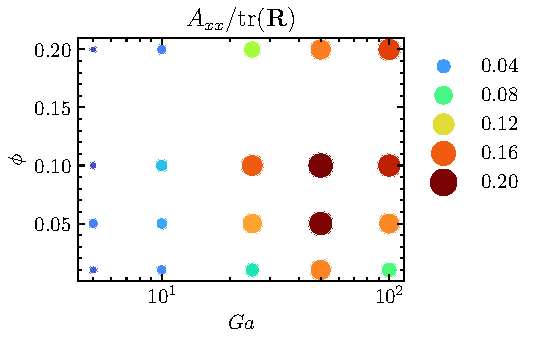
\includegraphics[height=5.5cm]{image/HOMOGENEOUS_NEW/PA/phase_axx_l_1.pdf}};
        \draw[dashed] (1.2,0.3) ellipse (1.5 and 2.5);
        \node (txt) at (1.2,1) {Anisotropic};
        \node (txt) at (-2,1) {Isotropic};

        \node (img) at (10.5,0) {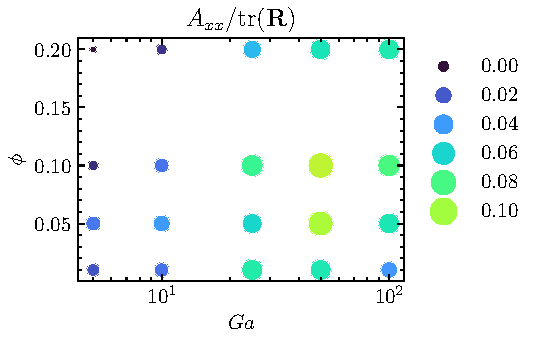
\includegraphics[height=5.5cm]{image/HOMOGENEOUS_NEW/PA/phase_axx_l_10.pdf}};
        % \draw[dashed] (11.7,-0.5) ellipse (0.75 and 1.75);
        % \node (txt) at (11.7,1) {Anisotropic};
        \node (txt) at (8,1) {Isotropic};
    \end{tikzpicture}
    \caption{
        (top) Phase diagram of the dimensionless mean square distance to the nearest neighbor, $\textbf{R}:\textbf{I}/r_m^2$.
        (bottom) Phase diagram of the dimensionless horizontal components of the anisotropy tensor, $A_{xx}/\text{tr}(\textbf{R})$.  
        (left) Iso-viscous emulsion $\lambda = 1$.
        (right) Viscous droplets $\lambda = 10$.
        Reprinted from \citet{fintzi2024buoyancy} }
    \label{fig:A}
\end{figure}


The steady state analysis of \textbf{R} have been performed in \citet{fintzi2024buoyancy} we now wish to study the kinematic aspect of this tensor. 
To that end we make use of the transport equation of $P_\text{nst}(\textbf{x},\textbf{r},t,a)$ derived in \citet{zhang2023evolution}.
As it is a new formalism we recall this equation here, 
\begin{equation}
    \pddt P_\text{nst}
    + \pdda P_\text{nst}
    + \pddx \cdot  (\textbf{u}^\text{nst}_p P_\text{nst})
    + \pddr \cdot  (\textbf{w}^\text{nst}_p P_\text{nst})
    = \delta(a)P(\textbf{x},\textbf{r},t,0)
    - \frac{P_\text{nst}(\textbf{x},\textbf{r},t,a)}{\tau^\text{nst}(\textbf{x},\textbf{r},t,a)}
    \label{eq:dt_Pnst}
\end{equation}
The left-hand side of \ref{eq:dt_Pnst} corresponds to the convective derivative of $P_\text{nst}$ with respect to the nearest particle statistics' coordinate, i.e. $(\textbf{x},\textbf{r},t,a)$. 
The first term on the right-hand side of \ref{eq:dt_Pnst} account for the creation of the nearest pairs, thus it is non-zero only for the age $a = 0$, as witnessed by the Dirac delta function $\delta(a)$. 
The second term on the right-hand side is the contribution from the destruction of the nearest pairs.
We defined $1/\tau^\text{nst}(\textbf{x},\textbf{r},t,a)$ as the rate of destruction of nearest neighbors of age $a$ with relative position $\textbf{r}$.
Additionally, we define the ensemble averaged rate of destruction as
\begin{equation}
    \frac{1}{\tau_p}(\textbf{x},t) = 
    \frac{1}{n_p(\textbf{x},t)}
    \int_{0}^\infty
    \int_{\mathbb{R}^3}
    \frac{P_\text{nst} }{\tau^\text{nst}}(\textbf{x},\textbf{r},t,a)
    da d\textbf{r}. 
    \label{eq:tau_p}
\end{equation}
As we show in the next few paragraphs, $\tau_p$ is of utmost importance as it governs the timescale of the microstructure.

Note that a given particle always posses a nearest neighbor.
Therefore, when a particle stop being the nearest neighbor of a given particle, another particle comes and becomes the new nearest neighbor to that particle.
This exchange of nearest neighbors takes place at a constant radial distance $r$ due to the definition of $h_{ij}(t,\FF)$ \citep{zhang2021ensemble}. 
As a result, the first and second terms on the right-hand side of \ref{eq:dt_Pnst} have no impact on the nearest neighbor radial distribution function. 
Based on this remark \citep{zhang2023evolution} could show that
\begin{equation}
    \int_{0}^{\infty}\oint_{\mathbb{R}^2}\left[
        \delta(a)P(\textbf{x},\textbf{r},t,a)
    - \frac{P_\text{nst}(\textbf{x},\textbf{r},t,a)}{\tau^\text{nst}(\textbf{x},\textbf{r},t,a)}
    \right]dS(r) da    
    =0,
    \label{eq:int_dt_h}
\end{equation}
where we integrated over a spherical shell of radius $r$, such that $dS(r)$ is an infinitesimal portion of this spherical shell. 
% That expression provides constancy between \ref{eq:dt_Pnst} and the transport equation of the number density. 
That expression will find its use in the following paragraphs. 


By taking the partial time derivative of \ref{eq:R}, and utilizing \ref{eq:dt_Pnst}, \ref{eq:u_p} and \ref{eq:tau_p} we obtain an equation for $\textbf{R}(\textbf{x},t)$, it reads,
\begin{equation*}
    \pddt (n_p\textbf{R})
    + \pddx \cdot [n_p(\textbf{u}_p\textbf{R}
    + \textbf{R}^\text{Re})]
    = 
    - \frac{n_p\textbf{R}}{\tau_p}
    +n_p\textbf{B}
    + n_p\textbf{D}
    + n_p\textbf{W}
    \label{eq:dt_R}
\end{equation*}
With,
\begin{align*}
    n_p \textbf{R}^\text{Re}(\textbf{x},t)
    =
    \int_{0}^\infty
    \int_{\mathbb{R}^3}
    \textbf{rr}(\textbf{u}^\text{nst}_p - \textbf{u}_p)
    P(\textbf{x},\textbf{r},t,a)
    d\textbf{r}da,\\
    n_p \textbf{B}(\textbf{x},t)
    =
    \int_{0}^\infty
    \int_{\mathbb{R}^3}
    \textbf{rr}
    P(\textbf{x},\textbf{r},t,0)\delta(a)
    d\textbf{r}da, \\
    n_p\textbf{D}(\textbf{x},t) = 
    \int_{0}^\infty
    \int_{\mathbb{R}^3} \textbf{rr}
    \left[
        \frac{1}{\tau_p(\textbf{x},t)}
        - \frac{1}{\tau^\text{nst}(\textbf{x},\textbf{r},t,a)}
    \right]
    P_\text{nst}
    d\textbf{r}
    da,\\
    n_p \textbf{W}(\textbf{x},t) = 
    \int_{0}^\infty
    \int_{\mathbb{R}^3} \left[
        \textbf{r} \textbf{w}^\text{nst}_p
        + \textbf{w}^\text{nst}_p\textbf{r}
    \right]P_\text{nst}
    d\textbf{r}
    da.
\end{align*} 
The tensor $\textbf{R}^\text{Re}$ represent the flux due to the velocity fluctuations. 
The source term $\textbf{B}$ is the averaged square relative position conditioned on the age $a=0$, meaning that it is related to the birth of the nearest particle pairs. 
In opposition to \textbf{D} which is related to the death of the particles pairs due to the presence of the terms $\tau_p$ and $\tau_p^\text{nst}$.
Therefore, $\textbf{B}$ is the weighted average of $\textbf{rr}$ on the Dirac distribution $\delta(a)$. 
Likewise, $\textbf{D}$ is the weighted average of $\textbf{rr}$ in terms of the destruction rate fluctuation field. 
The former term cancels out under the hypothesis that $1 / \tau^\text{nst}_p(\textbf{x},\textbf{r},t,a)$ is independent of age and relative position, in which case $\tau_p = \tau^\text{nst}_p$. 
This would imply that the odds for a nearest neighbor to be replaced by another particle is equally likely regardless of its current position \textbf{r} and age $a$. 
Such simplification might be valid at high particle velocity fluctuations in which case these events become \textit{random}.
In the DNS results presented in \ref{sec:velocity} we show that this simplification is not valid in the range of parameters investigated in this study.
Additionally, the tenor $\textbf{W}(\textbf{x},t)$ is the correlation between the particles relative position \textbf{r} and relative velocity $\textbf{w}_p^\text{nst}$.
Furthermore, due to the presence of the first term on the right-hand side of \ref{eq:dt_R}, we can state that $\textbf{R}(\textbf{x},t)$ will eventually relax within time, and that the relaxation time is $\tau_p$. 
In \citet{zhang2023evolution} they demonstrate that it is also the case for the particle-fluid-particle stress tensor.
In fact, this hold true for all nearest-neighbor averaged particles quantities, since this relaxation time is related to the transport equation of $P_\text{nst}(\textbf{x},\textbf{r},t,a)$, see \ref{eq:dt_Pnst}.
The main takeaway from \ref{eq:dt_R} is that, the microstructure as it is described by $\textbf{R}(\textbf{x},t)$, is motivated by 3 source terms, a term related to the weighted average of $\textbf{rr}$ on pair's birth and on pair's destruction, and a last one related to the particle relative velocity-position correlation. 


The knowledge of $\textbf{R}(\textbf{x},t)$ provides useful information to feed the closure terms in the Euler-Euler models.
For example, the value of the averaged interphase momentum transfer dependents on the instantaneous shape of the microstructure. 
Therefore, since $\textbf{R}(\textbf{x},t)$ follows a kinetic theory-like transport equation, it is interesting to discuss the possibility of implementing an equation such as \ref{eq:dt_R} in an Euler-Euler model. 
Of course this is useful only if one has explicit expressions of the closure terms present in the Euler-Euler model as a function of $\textbf{R}(\textbf{x},t)$, which is not currently the case.
Even so, attempting to solve \ref{eq:dt_R} directly is very challenging due to the presence of numerous unknown terms ($\textbf{R}^\text{Re}$, $\textbf{D}$, $\textbf{B}$ and $\textbf{W}$).
Instead, one could directly find an expression for $\textbf{R}(\textbf{x},t)$ as a function of the flow parameters based on the results of \citet{fintzi2024buoyancy}, which are statistically steady-state results of $\textbf{R}(\textbf{x},t)$. 
But then, how to know if the inertial effects related to the formation of the microstructure  (left hand-side of \ref{eq:dt_R}) are negligible ?
In fact, provided a relaxation time of the microstructure sufficiently small compared to the timescale of the macroscopic flow, the derivatives on the left hand-side of \ref{eq:dt_R} might be negligible.
Therefore, $\textbf{R}(\textbf{x},t)$ can be expressed directly in terms of the flow parameters, provided that $\tau_p$ is smaller than the flow timescale. 
Therefore, the time $\tau_p$ is of major importance for two reasons: 
(1) according to \ref{eq:dt_R} it determines the timescale at which a statistically steady microstructure might be reached; 
(2) it provides useful information in the modeling of \ref{eq:dt_R}.


